\documentclass[conference,10pt]{IEEEtran}

\usepackage{amsmath,amssymb,amsfonts}
\usepackage{graphicx}
\usepackage{booktabs}
\usepackage{cite}
\usepackage{xcolor}
\usepackage{hyperref}

\hypersetup{colorlinks=true,linkcolor=blue,citecolor=blue,urlcolor=blue}
\graphicspath{{../../figures/hyqad/}}
\renewcommand{\arraystretch}{1.1}

\title{Calibrated and Kernel-Based Detection of QKD\\Implementation Attacks in a Controlled Simulation}

\author{
  \IEEEauthorblockN{Arnav Kapoor}
  \IEEEauthorblockA{Department of Computer Science\\
  \textit{IISER Bhopal}\\
  Bhopal, India\\
  arnavkapoor23@iiserb.ac.in}
}

\begin{document}

\maketitle

\begin{abstract}
Machine-learning detectors for attacks on quantum key distribution (QKD) are
usually tested on simulated telemetry. Many report near-perfect accuracy. We
show that this can come from the simulator. Without drift in normal operation, a
single telemetry feature separates attacks perfectly. We build a seeded
decoy-state BB84 simulator with operating drift, finite-size noise and one
attack-strength parameter $s$. On it we compare a Gaussian-process classifier
(GP), an amplitude-encoding fidelity-kernel SVM (AE-SVM), an RBF-kernel SVM,
random forests and a stacked model. Every model is trained on the same data at
every training size. At $s=0.3$ all supervised models reach 0.80 to 0.84 MCC.
Random forests are best or tied best. The GP is the least calibrated model. It
also gives the worst uncertainty for deferring alerts. AE-SVM matches RBF-SVM.
It generalizes to unseen attack types only because one feature carries the
input's magnitude. Removing that feature drops its held-out AUC from 0.95 to
0.55. A one-coordinate norm anchor restores it to 0.94.
\end{abstract}

\begin{IEEEkeywords}
Quantum key distribution, anomaly detection, Gaussian processes, quantum kernels, calibration, simulation
\end{IEEEkeywords}

\section{Introduction}

QKD draws its security from physics~\cite{bennett1984quantum,gisin2002quantum}.
Real systems still leak through their hardware. Known attacks include
photon-number splitting (PNS)~\cite{huttner1995photon,lutkenhaus2002pns},
detector blinding~\cite{makarov2006effects,lydersen2010hacking}, Trojan-horse
probing~\cite{gisin2006trojan,jain2014trojan} and
intercept-resend~\cite{bennett1992experimental}.

Telemetry monitoring is one defense. Machine learning has been applied to
it~\cite{mao2020detecting} and to related QKD control tasks~\cite{ren2021machine}.
Two problems make such results hard to judge. Detectors are tested on simulated
telemetry, and a simulator with one fixed operating point makes most attacks easy
to spot. Quantum models are also often trained on fewer samples than the
baselines.

This paper is a controlled simulation study. Our contributions are as follows.
\begin{enumerate}
\item A seeded telemetry simulator with drift, leakage tests and an attack-strength
  axis $s$.
\item A comparison of five detectors trained on the same data at every size.
\item An explanation, confirmed by ablation, of when the amplitude kernel
  generalizes to unseen attacks.
\item Evidence that a recalibrated random forest gives better alert deferral than
  a GP posterior.
\end{enumerate}

\section{Telemetry Simulator}
\label{sec:sim}

Each sample is one key-generation block of a decoy-state BB84 link over 50\,km of
fiber. Let $\mu$ be the mean photon number, $T$ the transmittance and $\eta$ the
detector efficiency. A Poisson source then gives~\cite{lo2005decoy}
\begin{align}
Q_\mu &= Y_0 + \bigl(1-e^{-\eta T\mu}\bigr)(1+p_{\mathrm{ap}}),\\
E_\mu &= \bigl[\tfrac12 Y_0 + e_d\,(1-e^{-\eta T\mu})(1+p_{\mathrm{ap}})\bigr]/Q_\mu .
\end{align}
Here $Y_0$ is the dark-count probability, $e_d$ the misalignment error and
$p_{\mathrm{ap}}=0.005$ the afterpulse probability.

Normal operation drifts from block to block. Loss varies by 0.3\,dB and detector
efficiency by 3\%. Misalignment, dark counts and background light vary
log-normally. The two error-rate estimates carry finite-size noise for blocks of
5,000 bits. Each block reports seven measurements.

The four attacks perturb these measurements following their published
descriptions~\cite{huttner1995photon,makarov2006effects,gisin2006trojan,bennett1992experimental}.
The perturbation sizes are modeling assumptions. Every deviation is multiplied by
a strength $s$. At $s=1$ the attack uses its default size. As $s$ falls toward 0
it becomes indistinguishable from normal blocks (Fig.~\ref{fig:qber}).

\begin{figure*}[t]
  \centering
  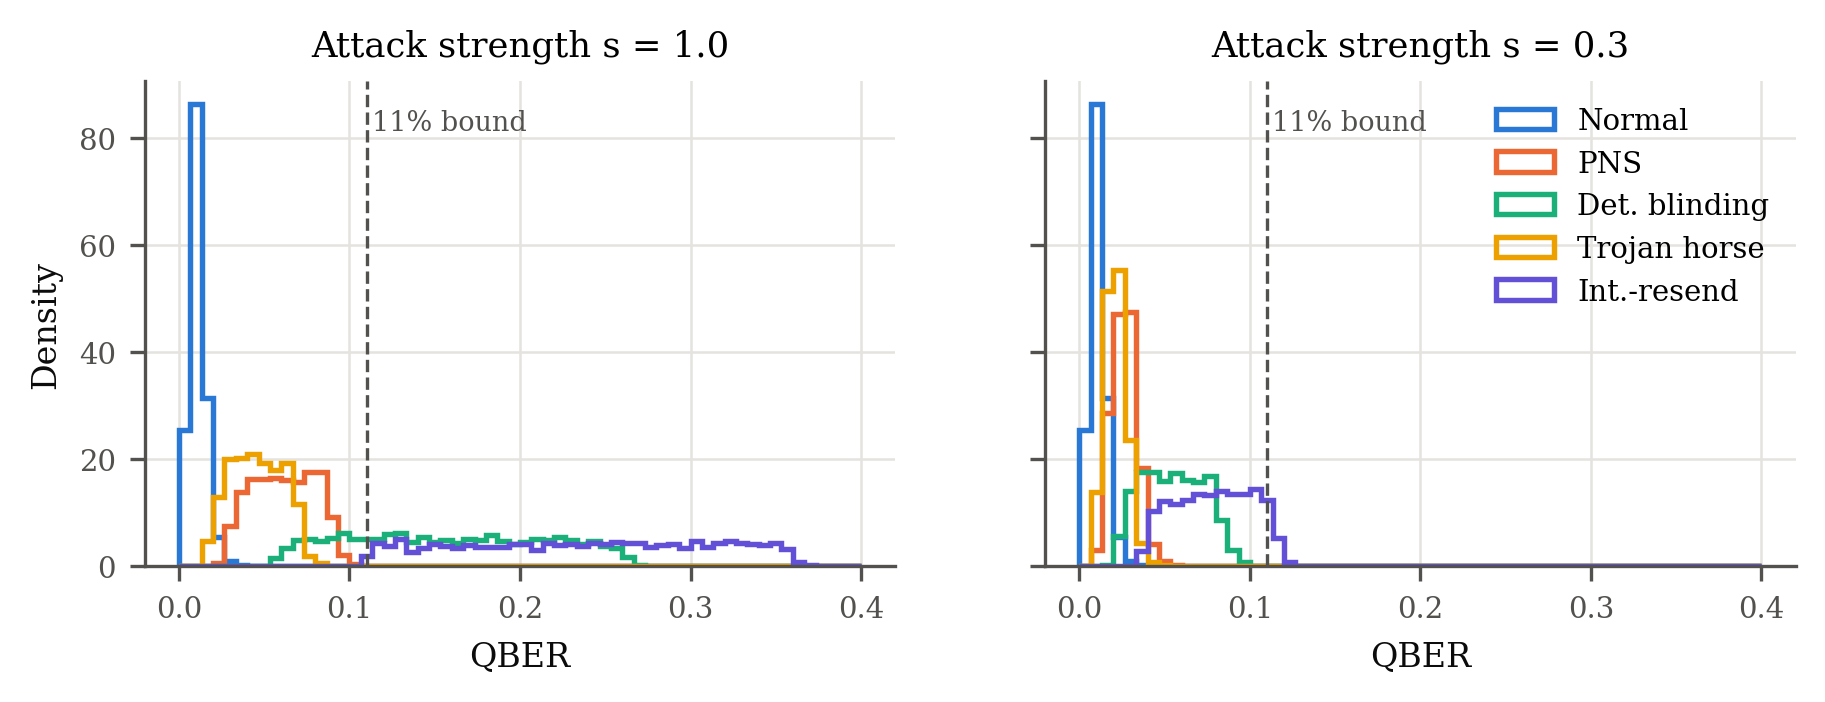
\includegraphics[width=0.8\textwidth]{fig2_qber_dist.png}
  \caption{QBER by class at $s=1$ and $s=0.3$. At $s=0.3$, PNS and Trojan-horse blocks overlap normal operation well below the 11\% bound.}
  \label{fig:qber}
\end{figure*}

We release two leakage tests with the simulator. Different seeds must give
different datasets. No single feature may act as a label. An earlier version of
our own pipeline failed both tests. There, the error rate alone separated
attacks perfectly and every model looked near-perfect.

\section{Detectors and Protocol}

\begin{figure*}[t]
  \centering
  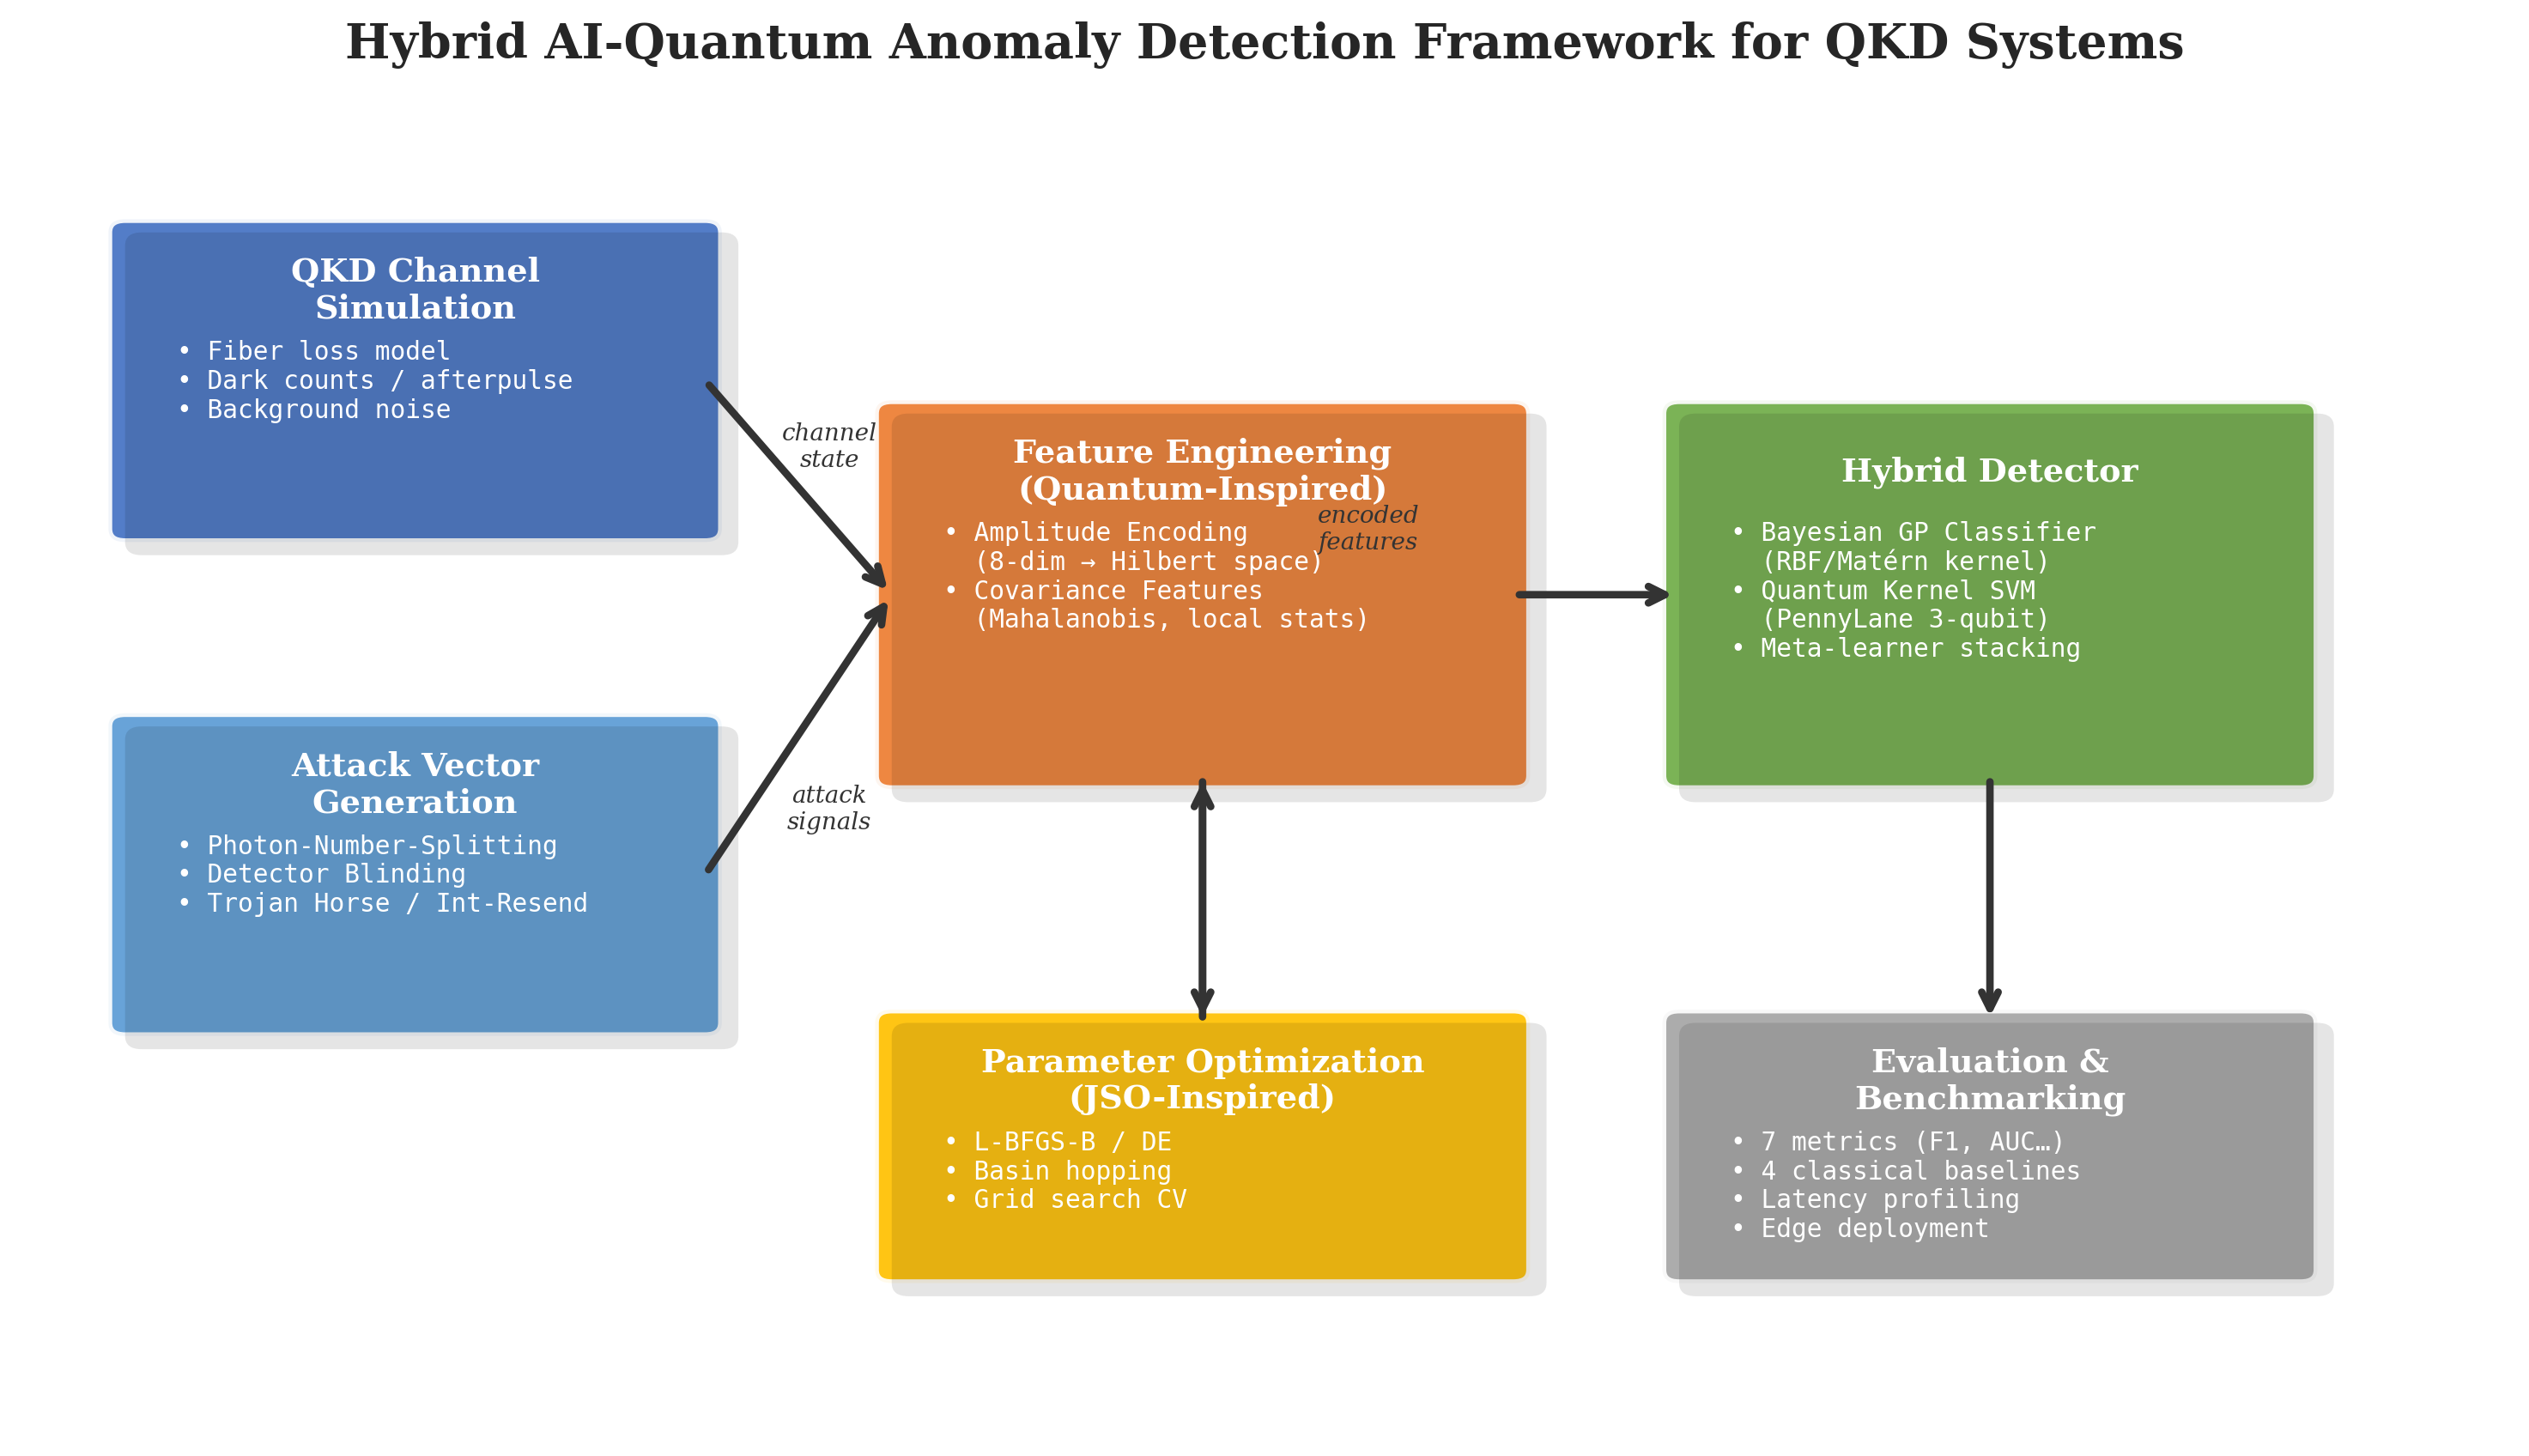
\includegraphics[width=\textwidth]{fig1_framework_hyqad.png}
  \caption{Study design. All detectors share one 8-dimensional feature map.}
  \label{fig:framework}
\end{figure*}

Every detector sees the same 8 features (Fig.~\ref{fig:framework}). These are
the 7 measurements standardized on the training data and a robust Mahalanobis
distance~\cite{rousseeuw1999fast} to normal training blocks.

AE-SVM pads a vector with zeros to $2^q$ entries and normalizes it. Its fidelity
kernel is
\begin{equation}
K_A(\mathbf{x},\mathbf{y}) = |\langle\psi(\mathbf{x})|\psi(\mathbf{y})\rangle|^2
= (\hat{\mathbf{x}}^{\mathsf{T}}\hat{\mathbf{y}})^2 .
\label{eq:ka}
\end{equation}
This is the squared cosine similarity. It is cheap to compute classically. A
PennyLane~\cite{bergholm2018pennylane} simulation of the overlap circuit agrees
with it to $7\times10^{-15}$. The circuit takes 26\,ms per kernel entry and the
closed form $3\times10^{-4}$\,ms. All 8 features fit on 3 qubits.

$K_A$ ignores the input's norm, since $K_A(c\mathbf{x},\mathbf{y})=K_A(\mathbf{x},\mathbf{y})$
for any $c\neq0$. A norm-anchored variant appends a constant $c$ before encoding.
We set $c$ to the median training norm.

The baselines are a Laplace GP~\cite{rasmussen2006gaussian} and an RBF-kernel SVM.
We also use random forests (RF, 200 trees)~\cite{breiman2001random}, both raw and
isotonic-calibrated~\cite{zadrozny2002transforming}. Hybrid stacks the GP and
AE-SVM~\cite{wolpert1992stacked}. Three novelty detectors are fit on normal data
only.

Each run uses 2,000 blocks with 30\% attacks and a 70/30 split. We repeat it over
10 seeds and report 95\% confidence intervals. Matched-size runs train every model
on the same subsample. Zero-day runs train on three attack types and test on the
fourth.

\section{Results}

\begin{table*}[t]
  \centering
  \caption{Detection at $n=1400$ (mean $\pm$ 95\% CI, 10 seeds). ECE uses 15 bins. Bold marks the best supervised value per column.}
  \label{tab:bench}
  \footnotesize
  \begin{tabular}{lcccccc}
    \toprule
    & \multicolumn{3}{c}{$s=1.0$} & \multicolumn{3}{c}{$s=0.3$} \\
    \cmidrule(lr){2-4}\cmidrule(lr){5-7}
    Model & MCC & AUC & ECE & MCC & AUC & ECE \\
    \midrule
@HY_T_BENCH@
    \bottomrule
  \end{tabular}
\end{table*}

\subsection{In-distribution detection}

At $s=1$ every supervised model passes 0.95 MCC (Table~\ref{tab:bench}). This
setting cannot tell the methods apart. At $s=0.3$ the models spread from 0.80 to
0.84 MCC. RF, isotonic RF and Hybrid lead.

The GP has the lowest attack recall at $s=0.3$, 0.78 against 0.85 for RF and
0.90 for AE-SVM. It trades recall for specificity. Hybrid fixes 154 GP errors
and adds 76 across all seeds. Its gain is significant (McNemar) on 4 of 10
seeds. AE-SVM and RBF-SVM never differ significantly at $s=0.3$.

\begin{table}[t]
  \centering
  \caption{MCC at matched training size $n$ (mean of 10 seeds).}
  \label{tab:matched}
  \footnotesize
  \setlength{\tabcolsep}{4pt}
  \begin{tabular}{llcccc}
    \toprule
    $s$ & Model & $n=25$ & 100 & 500 & 1400 \\
    \midrule
@HY_T_MATCHED@
    \bottomrule
  \end{tabular}
\end{table}

\subsection{Training size and attack strength}

RF learns fastest at both strengths (Table~\ref{tab:matched}). AE-SVM needs more
data than RBF-SVM to reach the same MCC. It is never reliably ahead. Hybrid is
unstable at $n=25$, where its stacking folds hold only 8 blocks each.

\begin{table}[t]
  \centering
  \caption{MCC against attack strength $s$ at $n=1400$, and GP recall per attack type.}
  \label{tab:strength}
  \footnotesize
  \setlength{\tabcolsep}{3pt}
  \begin{tabular}{lcccccc}
    \toprule
    $s$ & 0.05 & 0.1 & 0.2 & 0.3 & 0.5 & 1.0 \\
    \midrule
@HY_T_STRENGTH@
    \bottomrule
  \end{tabular}
\end{table}

All four detectors fall together as $s$ shrinks (Table~\ref{tab:strength}). RF
leads for $s\ge0.2$. Below that the models are within 0.04 MCC of each other.
Blinding and intercept-resend stay visible down to $s=0.1$ because they raise
QBER the most. PNS and Trojan-horse probing are lost first.

\subsection{Unseen attack types}

\begin{table}[t]
  \centering
  \caption{AUC on a held-out attack type at $s=0.3$ (10 seeds). The last column removes the Mahalanobis feature.}
  \label{tab:zd}
  \footnotesize
  \setlength{\tabcolsep}{2.5pt}
  \begin{tabular}{lcccccc}
    \toprule
    Model & PNS & Blinding & Trojan & Int.-res. & Mean & No Mahal. \\
    \midrule
@HY_T_ZD@
    \bottomrule
  \end{tabular}
\end{table}

\begin{figure}[t]
  \centering
  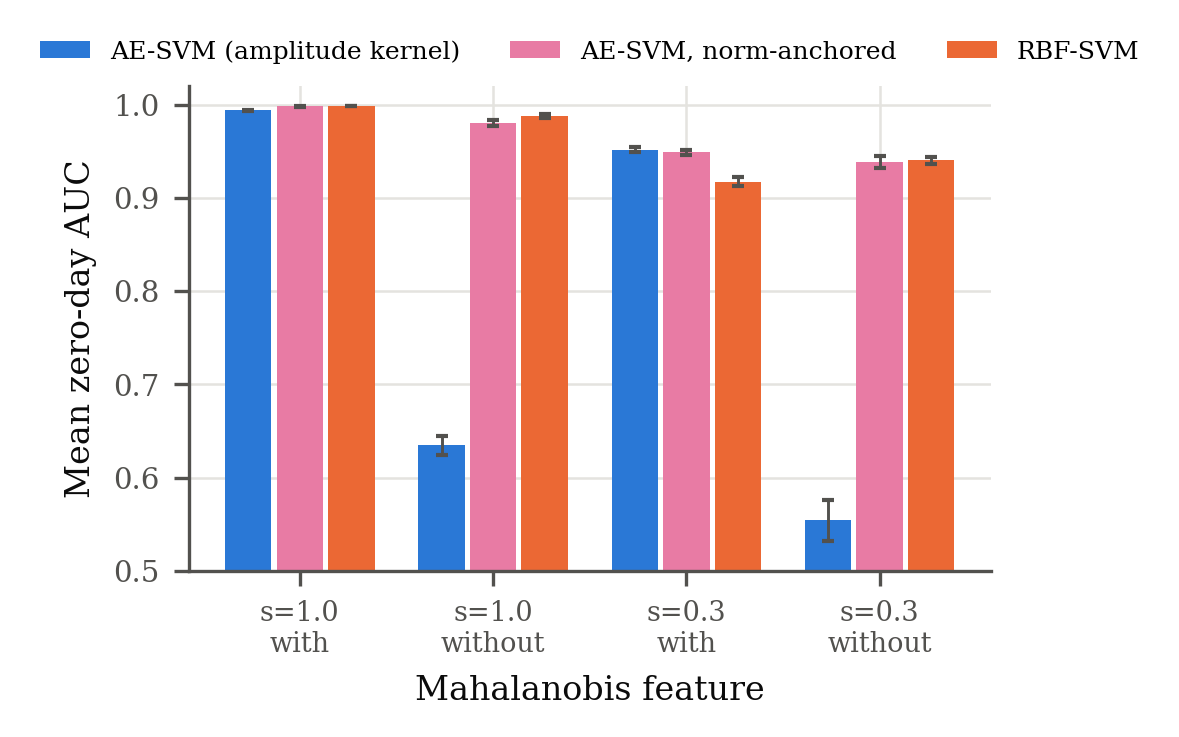
\includegraphics[width=0.95\columnwidth]{fig9_mahal_ablation.png}
  \caption{Mean held-out AUC with and without the Mahalanobis feature.}
  \label{fig:mahal}
\end{figure}

AE-SVM generalizes nearly as well as RF and better than RBF-SVM (Table~\ref{tab:zd}).
This is surprising, because its kernel-target
alignment~\cite{cristianini2002kernel} is lower. It is 0.13 to 0.22 against 0.29
to 0.66 for RBF.

The explanation is Eq.~\eqref{eq:ka}. $K_A$ ignores the norm, but an unseen
attack is easiest to spot by how far it sits from normal blocks. In our features
that distance is carried by one coordinate, the Mahalanobis distance. Removing it
drops AE-SVM to 0.554 at $s=0.3$ and 0.635 at $s=1$ (Fig.~\ref{fig:mahal}).
RBF-SVM is unaffected. The norm anchor restores AE-SVM to 0.939 and 0.980.

\begin{table}[t]
  \centering
  \caption{Accuracy on control tasks in $\mathbb{R}^8$ with heavy-tailed norms (10 seeds).}
  \label{tab:cross}
  \footnotesize
  \setlength{\tabcolsep}{3pt}
  \begin{tabular}{lrcccc}
    \toprule
    Label depends on & $n$ & AE-SVM & RBF-SVM & GP & RF \\
    \midrule
@HY_T_CROSS@
    \bottomrule
  \end{tabular}
\end{table}

Table~\ref{tab:cross} isolates this bias. When labels depend on direction only,
AE-SVM learns from far fewer samples than any baseline. When labels depend on
norm only, it stays at chance. QKD telemetry lies between these extremes.

\subsection{Calibration and deferral}

\begin{figure*}[t]
  \centering
  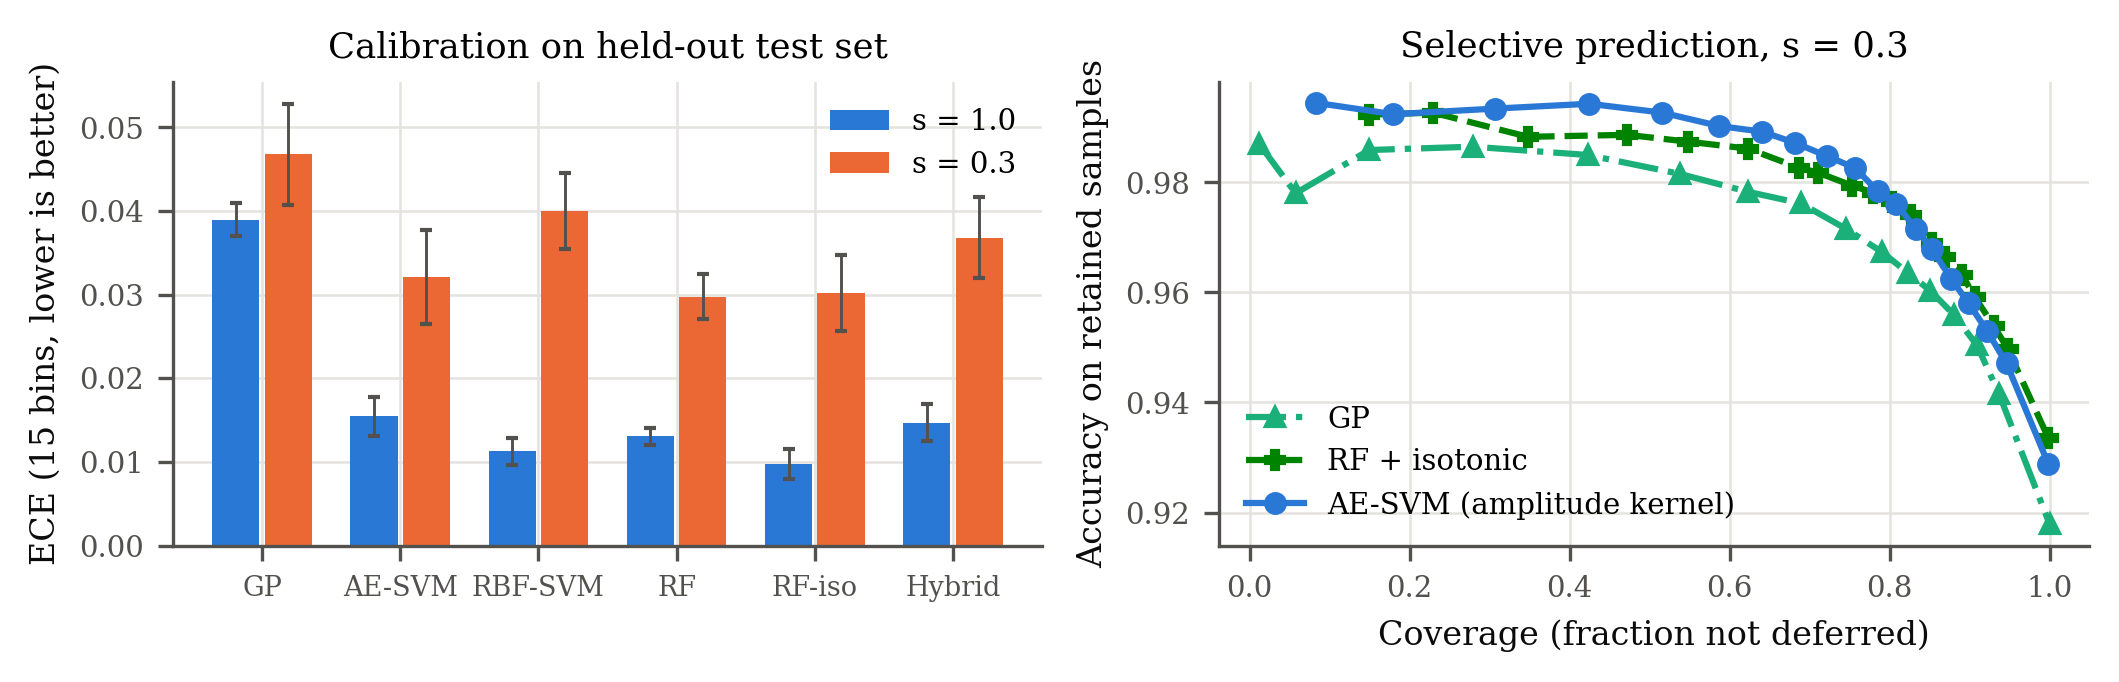
\includegraphics[width=0.8\textwidth]{fig6_calibration_selective.png}
  \caption{Left, ECE by model. Right, accuracy against coverage when blocks with uncertainty $u=\sqrt{p(1-p)}$ above a threshold are deferred ($s=0.3$).}
  \label{fig:calib}
\end{figure*}

\begin{table}[t]
  \centering
  \caption{Deferral at $s=0.3$. Coverage is the share of blocks kept, and accuracy is measured on those blocks.}
  \label{tab:select}
  \footnotesize
  \setlength{\tabcolsep}{4pt}
  \begin{tabular}{lcccc}
    \toprule
    & \multicolumn{2}{c}{$u<0.3$} & \multicolumn{2}{c}{$u<0.1$} \\
    \cmidrule(lr){2-3}\cmidrule(lr){4-5}
    Model & Coverage & Accuracy & Coverage & Accuracy \\
    \midrule
@HY_T_SELECT@
    \bottomrule
  \end{tabular}
\end{table}

The GP is the least calibrated supervised model, and isotonic RF the best
(Table~\ref{tab:bench}, Fig.~\ref{fig:calib}). The GP's probabilities crowd the
decision boundary. At $u<0.3$ it keeps fewer blocks than isotonic RF or AE-SVM at
the same accuracy (Table~\ref{tab:select}). At $u<0.1$ it keeps none. On this data
a recalibrated point estimate makes the better deferral policy.

\subsection{Evasion and cost}

\begin{table}[t]
  \centering
  \caption{Evasion at $s=0.3$. The five most important features of each attack block move toward the normal median by the given budget.}
  \label{tab:adv}
  \footnotesize
  \begin{tabular}{lccc}
    \toprule
    Budget & RF detection & GP detection & GP uncertainty \\
    \midrule
@HY_T_ADV@
    \bottomrule
  \end{tabular}
\end{table}

\begin{table}[t]
  \centering
  \caption{Inference cost on one CPU core, training excluded. Batch cost is per block over 600 blocks. Single-block cost is dominated by Python call overhead.}
  \label{tab:latency}
  \footnotesize
  \begin{tabular}{lcc}
    \toprule
    Component & Batch (ms) & Single (ms) \\
    \midrule
@HY_T_LAT@
    \bottomrule
  \end{tabular}
\end{table}

A simple evasion lowers RF and GP detection together (Table~\ref{tab:adv}). RF
stays 2 to 9 points ahead. The GP's uncertainty barely moves, so it does not flag
the evasion. Every detector runs far below a per-block budget measured in seconds
(Table~\ref{tab:latency}).

\section{Limitations}

Every result is simulated. The attack sizes are assumptions, and the drift model
is not fitted to a real link. The strength axis shows how results move with
signature size. It does not say which $s$ a real attacker produces. The evasion is
gradient-free and not adaptive. The detectors see single blocks, and models over
block sequences may do better. Testing on a physical QKD testbed is the next step.

\section{Conclusion}

On a simulator built not to be trivially separable, random forests are the
strongest and fastest-learning detector. Isotonic calibration gives better
deferral than a GP posterior. The amplitude kernel is competitive but not better.
It generalizes to unseen attacks only when some feature carries magnitude, and a
norm anchor supplies this when none does. Simulation studies of QKD detection
should report single-feature separability and a strength sweep alongside
accuracy.

\section*{Code and Data Availability}
Simulator, models, experiment scripts and all result files are at
\url{https://github.com/arnavk23/quasar-security}.

\bibliographystyle{IEEEtran}
\bibliography{../references}

\end{document}
